\chapter{ユーザスタディ}
\label{chap:visualize}

本章では開発したスマートフォンアプリDreamDateを用いたユーザスタディとその結果について述べ、提案手法の長所及び短所について考察する。

\section{予備実験1:音刺激の有無}
寝る前の10分間とレム睡眠中に曲を流すことが夢に影響を与えるか否かを検証するため予備実験を行った。スマートフォンは充電をした状態で枕の横に置くことで音が脳に届く状態にした。また睡眠を始める前に5分間海の夢が見たいと被験者に念じてもらった。\\
 20代後半女性の被験者A、40代後半女性の被験者Bと、20代前半女性の被験者Cに海の音を聞く日と効かない日を交互に14日間続けてもらうことで音が夢に影響を与えるのか否かの記録を行った。14日間の実験を行ったのは睡眠に関する実験は体調その日の活動内容や被験者の心境によって左右され、データーが変動しやすいためである。図\ref{experiment1}が実験スケジュールと実験結果である。青のハイライトがある日が関連する夢を見た日である。音が無い場合に被験者が海の夢を見たのは1回なのに対し、海の音を流して海の夢を見たのは4回であった。\\
 夢の具体的な内容について実験後インタビューをした。すると3日間夢を見たと答えた被験者Aは音のインプットが無い日は会社で働いている夢を見ることが多く、音を流しながら寝た日は10日ほど前に行った沖縄旅行での夢を見たと答えた。一度も海に関連した夢を見なかった被験者Bは海の音で起こされたりしたため、音は流れていたが全く関係の無い夢を見たと答えた。被験者Cは実験の最後の方で1年前に旅行したアメリカ西海岸に関する夢を見たと答えた。

\begin{figure}[htbp]
\begin{center}
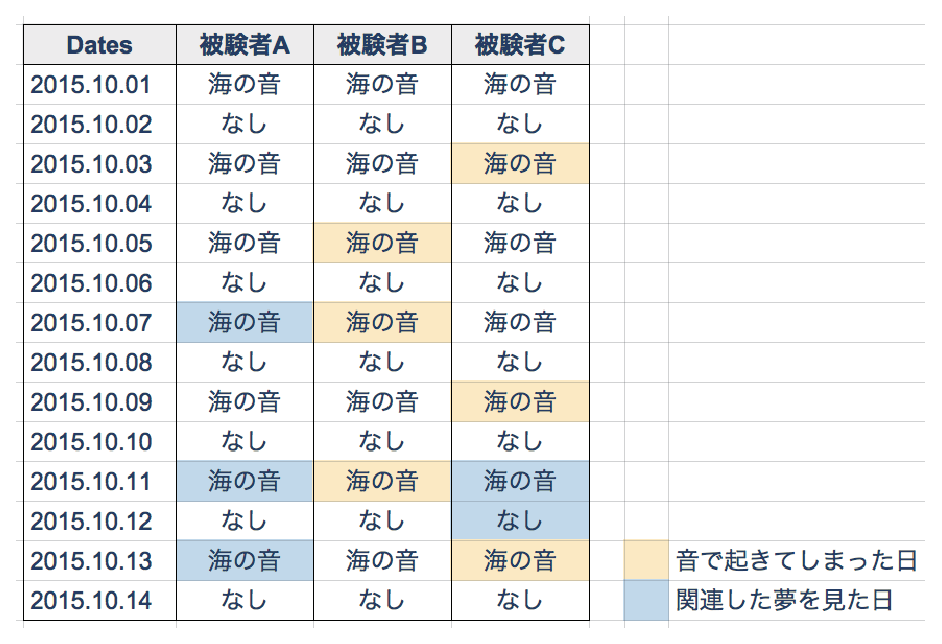
\includegraphics[width=13cm]{eps/schedule0.eps}
\caption{予備実験1:実験スケジュールと実験結果}
\label{experiment1}
\end{center}
\end{figure}

\section{予備実験2:音刺激の種類}
 どのような音がDreamDateに適しているのかを調べるために予備実験を行った。2年前から遠距離恋愛中の交際相手とデートをしている夢を見たいと望む被験者Cに「音声」、「曲」と「自然音」の3種類の音を試した。被験者Cの場合は「音声」は交際相手が被験者Cの名前を語りかけ、過去のデートの思い出話や、理想のデートの話しや、愛の言葉をささやくといった内容であった。「曲」は交際相手が被験者Cのために作曲と演奏した曲で、被験者Cも毎日通学で聞いている曲である。「自然音」はアメリカ西海岸の海で交際相手と共に聞いた波の音。図\ref{experiment2}が実験スケジュールと実験結果である。被験者の希望であった遠距離恋愛中の交際相手とデートしたいという要望を実現させることができたのは「曲」であった。\\
 夢の具体的な内容について実験後インタビューをした。関連する夢を見たのは「曲」と「自然音」のときである。11月9日は日本で再開する夢をみて、11月13日は江ノ島で友人と遊ぶ夢をみた。11月15日は交際相手から手紙が届く夢を見た。また、実験の結果から語りかけ口調の音声は被験者を毎回起こしてしまった。比べて波の音などの自然音や音楽は比較的被験者を1度しか起こさなかった。

\begin{figure}[htbp]
\begin{center}
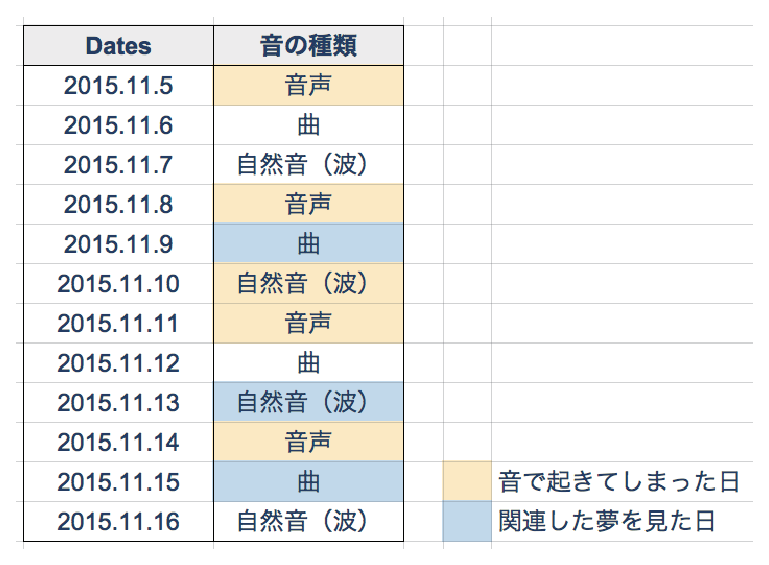
\includegraphics[width=13cm]{eps/schedule1.eps}
\caption{予備実験2:実験スケジュールと実験結果}
\label{experiment2}
\end{center}
\end{figure}

\section{予備実験から浮かび上がった仮説}
 予備実験1を経て同じ海の波の音でも結果に個人差が出るということがわかった。その理由として考えられるのがまず年齢である。Zhangは高齢になるにつれてレム睡眠の間隔が短くなると述べている\cite{Zhang}。次に考えられるのが被験者がどれだけそれに関連した夢を見たいと感じているかである。海の音を流した夜、被験者には全員海の夢を見たいと念じながら寝るようにと伝えたが、本心として海の夢を見たいと思っていたのは被験者Aと被験者Cのみであった。夢に対する希望が大きいほど、夢を見る確率が上がる可能性がある。他にも要素として考えられるのが、音と被験者の記憶との関連度だ。実験を行った後にそれぞれの被験者にどのような夢を見たかインタビューをした。すると海の夢を見た被験者 A と被験者 C はどちらも過去に海に行った際の思い出を夢見たと答えた。一方で 海にしばらく行っていない被験者 B は一度も海の夢を見なかった。この結果は被験者の記憶と関連性の高い音を流すと効果が出やすいということが示唆する。言い換えると印象に残っていない 体験や情景を DreamDate を使っても夢で再現することは困難である可能性がある。最後にどDreamDateの使用日数が結果に影響を与える可能性がある。というのは被験者Aと被験者Cは共に実験の前半に比べて実験後半の方が夢をみる確率が上がっているからである。明晰夢習得へのステップであるThe MILD Techniqueでも訓練を長く続ければ続けるほど、成功率があがると紹介されていることからDreamDateもな学使えば使うほど効果が出やすい可能性が高い\cite{LaBerge}。

予備実験から明晰夢に影響を与える可能性のある要素を以下に提示する
\begin{itemize}
\item 仮説1 : 年齢
\item 仮説2 : その夢を見たいと思う気持ちの強さ
\item 仮説3 : 思い出に関連した曲か否か(どれくらい印象に残っているか・いつの思い出か)
\item 仮説4 : DreamDateの使用期間
\end{itemize}

\section{実験: 音とタイミング}
 予備実験から浮かび上がった仮説を検証するために再度7名の被験者を対象に実験を行った。まず仮説1を検証するために被験者は20代、30代、40代と50代の人々を集めた。仮説2に基づいてすべての被験者に本当に見たい夢の内容を最初にインタビューし、その思い出に由来する音を聞き出しDreamDateに反映した。加えて寝る前に音楽を聴きながら思い出に関する画像を5分間眺めること、思い出について考えならが寝る意識をしてもらった。仮説3を明らかにするために頃の記憶か、直接的な記憶なのか、間接的な記憶なのかを事前にインタビューで聞き出し、証するための材料とした。仮説4を明らかにするために15日間実験を行い、時間の経過と実験結果に相関性があるかを検証した。\\
 加えて6時間以上睡眠を取れる日にのみ実験に参加してもらった。また被験者にはThe MILD Techniqueに基づいて夢を記憶できる体質になってもらうために実験を開始する5〜10日間前から、被験者には夢日記を書いてもらった。予備実験1と2では被験者が音に起こされてしまうという事態が発生したので本実験では、レム睡眠中ずっとと起きる直前のレム睡眠のみに音を流す場合をそれぞれ検証した。具体的には1 日目は音楽なし、2 日目はレム睡眠中音楽あり、3 日目は起きる直前のレム睡眠中音楽ありというを繰り返し 5 回、合計 15 日間続けてもらった。

\subsection{被験者の詳細と使用した音}
20歳〜50歳の男女、明晰夢に興味がある7人に参加してもらった。DreamDateは日本人のみならず、全世界のユーザを対象として制作しているので国籍と性別共に多様性のある被験者を集めた。また比較的安定したの睡眠活動をしている人を対象にした。下記に具体的な被験者の情報と使用する音を提示する。\\

被験者1:
\begin{itemize}
\item 国籍:インドネシア人
\item 性別:男性
\item 年齢:30代後半
\item 明晰夢の経験:5回ほど
\item 夢日記を付けた日数:5日間
\item 思い出に由来する音楽:被験者1は音楽にあまり関心がなく、特に思い出に残る音・音楽がなかった。そこで日常生活の中で音の刷り込みをした。具体的には実験10日間前から毎日コーヒーを飲むときにEdith Piafによる"Non je ne regrette rien"という曲。この音楽は映画inceptionの中で夢から覚めるために主人公たちが聴く音楽としても知られている。
\end{itemize}

被験者2:
\begin{itemize}
\item 国籍:日本人
\item 性別:女性
\item 年齢:40代後半
\item 明晰夢の経験:なし
\item 夢日記を付けた日数:10日間
\item 思い出に由来する音楽:被験者2は30年ほど前の結婚式で流した音楽 The CarpentersによるWe've only just begun
\end{itemize}

被験者3:
\begin{itemize}
\item 国籍:日本人
\item 性別:男性
\item 年齢:50代前半
\item 明晰夢の経験:なし
\item 夢日記を付けた日数:10日間
\item 思い出に由来する音楽:被験者3は007の映画を体験したいということだった。映画の中で使われているサウンドトラック
\end{itemize}

被験者4:
\begin{itemize}
\item 国籍:アメリカ人
\item 性別:男性
\item 年齢:20代前半
\item 明晰夢の経験:5回以上
\item 夢日記を付けた日数:5日間
\item 思い出に由来する音楽:被験者4は宮崎駿の映画である「魔女の宅急便キキ」を体験したいということだった。映画の中で使われているサウンドトラック
\end{itemize}

被験者5:
\begin{itemize}
\item 国籍:日本人
\item 性別:女性
\item 年齢:20代後半
\item 明晰夢の経験:なし
\item 夢日記を付けた日数:5日間
\item 思い出に由来する音楽:被験者5は今年の9月に社会人ダンス部でダンスを披露したときに利用したCell Block Tangoという曲
\end{itemize}

被験者6:
\begin{itemize}
\item 国籍:アメリカ人
\item 性別:男性
\item 年齢:20代前半
\item 明晰夢の経験:5回ほど
\item 夢日記を付けた日数:5日間
\item 思い出に由来する音楽:高校時代に演奏したバンドの曲、Fountains of WayneによるStacy's Momという曲
\end{itemize}

被験者7:
\begin{itemize}
\item 国籍:アメリカ人
\item 性別:男性
\item 年齢:20代後半
\item 明晰夢の経験:5回以上
\item 夢日記を付けた日数:5日間
\item 思い出に由来する音楽:1年前に交際相手のために作曲・演奏した曲Love From The Other Side Of The World\end{itemize}

\subsection{実験結果}
図\ref{experiment3}は実験のスケジュールと実験結果である。結論から述べると被験者7人が全員1回以上関連する夢を見ることができた。また予備実験1と本実験の結果から10人中8人が、音で刺激を与えた夜の方が与えなかった夜に対して明晰夢を見る確率が高かった。図\ref{musciOnNo}がその実験結果をまとめたものである。

\begin{figure}[htbp]
\begin{center}
\includegraphics[width=13cm]{eps/schedule2.eps}
\caption{実験スケジュールと実験結果}
\label{experiment3}
\end{center}
\end{figure}

\begin{figure}[htbp]
\begin{center}
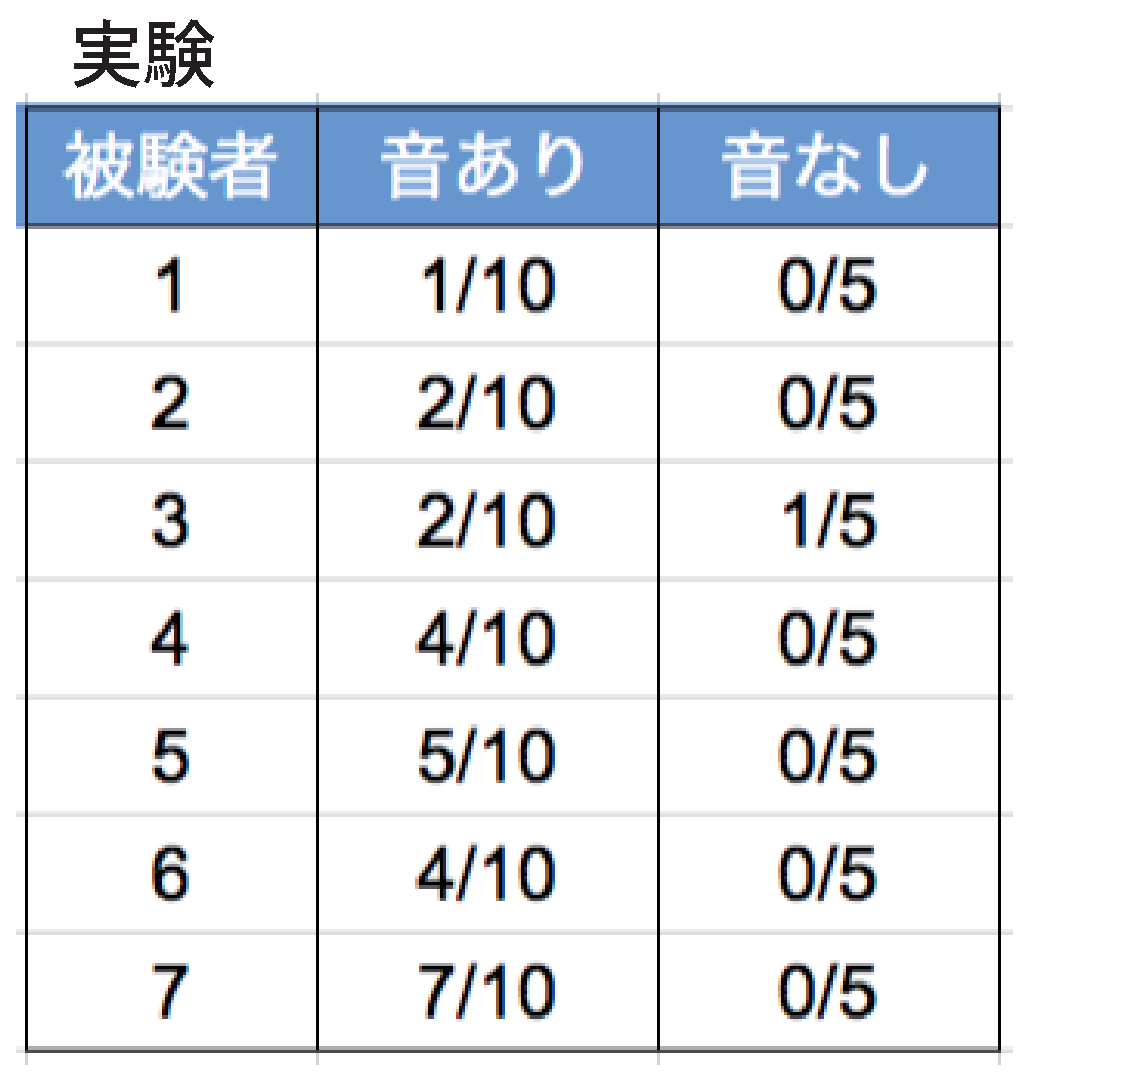
\includegraphics[width=13cm]{eps/musicOnNO.eps}
\caption{音有無の結果}
\label{musciOnNo}
\end{center}
\end{figure}

そこで予備実験を経て浮かび上がった、明晰夢に影響を与える可能性のある要素ごとに実験結果を図\ref{categorizedData}にまとめた。被験者1、被験者2、被験者5、被験者6、被験者7は直接的な体験であるのに対して、被験者3と被験者4は映画を通した間接的な思い出なので間接的と分類した。また思い出から経過している期間も記載した。

\begin{figure}[htbp]
\begin{center}
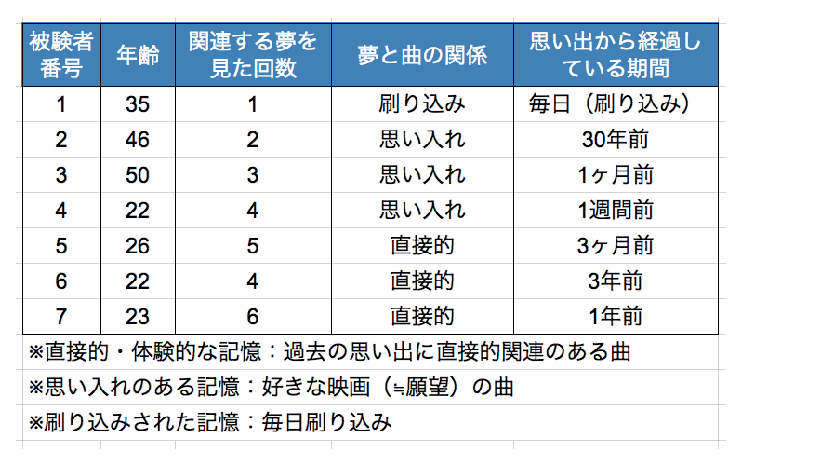
\includegraphics[width=13cm]{eps/categorizedData.eps}
\caption{実験結果のまとめ}
\label{categorizedData}
\end{center}
\end{figure}

図\ref{age}は被験者の年齢と関連する夢を見た回数の相関性を表す図である。直接的な思い出に関連した曲を聴いて寝た被験者は平均的に3.6回夢を見た。比べて間接的な思い出に関連した曲を聴いて寝た被験者は平均的に3.5回夢を見た。加えて予備実験前半に比べて後半の方が夢を見た回数が多いということが図\ref{experiment3}から読み取れる。

\begin{figure}[htbp]
\begin{center}
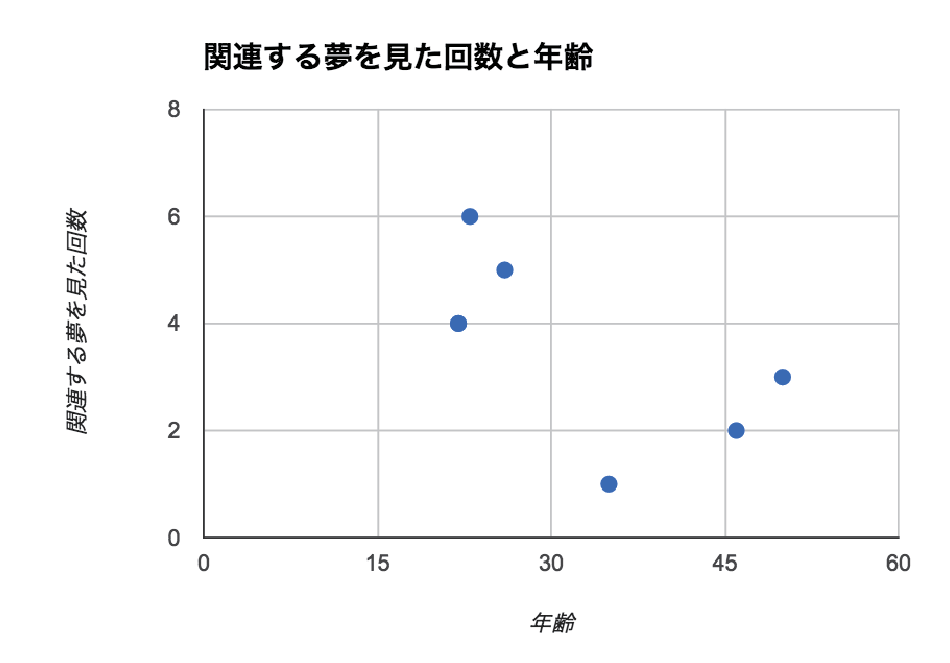
\includegraphics[width=12cm]{eps/age.eps}
\caption{被験者の年齢と関連する夢を見た回数}
\label{age}
\end{center}
\end{figure}

また音の影響によって7人の被験者のうち3人が起きてしまう事態が発生することが分かった。図\ref{result}は音楽を流したタイミング別に結果を表したグラフである。全ての被験者の実験結果を合計しタイミング別に関連した夢を見たときの確率を導き出した。音を流さないときは1/35、レム睡眠中ずっと音を流したときは10/35、そしてレム睡眠中に夢を見たときは13/35の確率で関連する夢を見た。

\begin{figure}[htbp]
\begin{center}
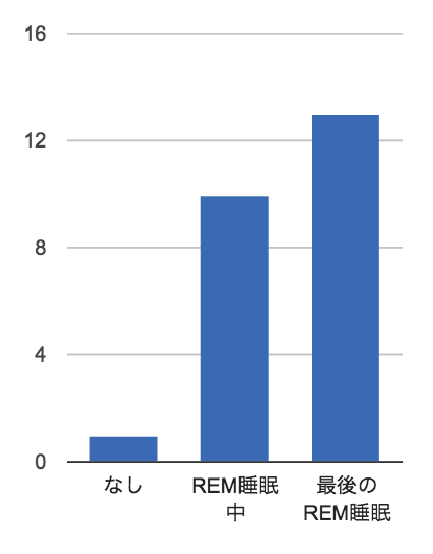
\includegraphics[width=6cm]{eps/result.eps}
\caption{刺激提示のタイミング別の関連した夢を見た回数}
\label{result}
\end{center}
\end{figure}

\section{考察}  
 本論文では研究の目的を
\begin{itemize}
\item 検証1: DreamDateによる明晰夢システムの有効性
\item 検証2: 明晰夢で好ましい仮想体験を味わうことはできるのか
\end{itemize}
と設定したが予備実験と実験結果からこれらについて関連する事象について考察を行う。

\subsection{DreamDateによる明晰夢システムの有効性} 
被験者7人が全員1回以上関連する夢を見ることができた。また予備実験1と本実験の結果から10人中8人が、音で刺激を与えた夜の方が与えなかった夜に対して明晰夢を見る確率が高かった。図\ref{musciOnNo}を参照。この結果はDreamDateの明晰夢システムとしての有効性を示す。

ただ結果には明らかに個人差があった。予備実験から浮かび上がった仮説が
\begin{itemize}
\item 仮説1 : 年齢
\item 仮説2 : その夢を見たいと思う気持ちの強さ
\item 仮説3 : 思い出に関連した曲か否か(どれくらい印象に残っているか・いつの思い出か)
\item 仮説4 : DreamDateの使用期間
\end{itemize}
だったため、それぞれの仮説の検証について述べる。

 実験後「年齢」がDreamDateの効果に影響を与えているか否かに関しては、30歳以下の被験者は平均的に4.75回明晰夢を体験したのに対して、30歳以上の被験者は平均的に2回明晰夢を体験したという結果から、年齢が上がるに連れて明晰夢を体験しにくい体質になる可能性がある。しかし被験者の数が少なすぎて図\ref{age}のグラフからは年齢と結果に相関性を見ることはできなかったため、被験者を増やしてもう一度実験をする必要がある。\\
 実験では「その夢を見たいと思う気持ちの強さ」がDreamDateの効果に影響を与えているか否かに関しては検証できなかった。それはそれぞれの被験者がどのくらいその夢を見たいかを数値的に計ることが難しかったからである。再度実験を行う場合は事前に明晰夢に対する期待度を数値化する必要があるだろう。例えば、「夢をすごく見たい」「夢を見れたら嬉しい」「夢を見れなくてもまぁ仕方ない」のどれかを選んでもらい、実験結果と期待度に壮観がるか否かを検証する必要がある。\\
 「思い出関連した曲か否か」がDreamDateの効果に影響を与えているか否かに関してはある程度検証できた。実験結果によると自ら作曲した歌、演奏した曲、ダンスをした曲などの直接的な記憶にを連想させる音楽を流した被験者5(3ヶ月前にダンスを披露したときの音楽を流した)と被験者6(3年前にバンドで演奏したときの音楽を流した)と被験者7(1年前に作曲した音楽を流した)は10/30の確率で関連性のある夢を見た。次に過去の思い出に関連した音楽を流した被験者1(毎日コーヒーを飲む際の音楽を流した)と被験者2(30年前の結婚式のときの音楽を流した)は3/30の確率で関連性のある夢を見た。一方実際に自分は体験していないが映画などを通して間接的に体験した記憶にまつわる音楽を流した被験者3(1ヶ月前に見た映画の音楽を流した)と被験者4(1週間前に見た映画の音楽を流した)は7/30の確率で夢を見た。図\ref{experiment3}を参照。この結果は流す音がユーザにとって直接的な体験ほど夢に影響を与えやすいということを示唆している。Zhangは夢は記憶の整理をするために見るものだと述べている\cite{Zhang}。被験者Aの場合波の音が過去の記憶を思い出させる音を流すことがトリガーとなり、脳が反応し思い出が夢として再生されたと考えられる。第2章で紹介したDreamOnやユメミールなどのスマートフォンアプリケーションは「鳥の音で森林にいる夢をみることができる」、「貨幣が落ちる音でお金持ちになる夢をみることができる」、「拍手の音で表彰される夢をみることができる」、「フライパンでベーコンが焼ける音で朝食の夢をみることができる」と説明している。しかしユーザはそれぞれ違った経験の持ち主なので全てのユーザにその効果が現れるかの見解には再考の余地が残る。株式会社タカラトミーのホームページでも夢見工房の効果に関しては個人差があると紹介している。その理由もユーザによって音や香りとそれまでの記憶との関連性が違うからだと推測することができる。\\
 「DreamDateの使用期間」については仮設通り、試用期間が長くなるにつれて成功確率が上がったことが図\ref{dates}からわかる。この図はでは図\ref{experiment3}の結果からDreamDateを使用しなかった日数を除いてグラフにした。よって合計10日間の実験と明晰夢を見た被験者の人数の相関図である。被験者の数が少ないので人数を増やしてもう一度実験をする必要がある。
\begin{figure}[htbp]
\begin{center}
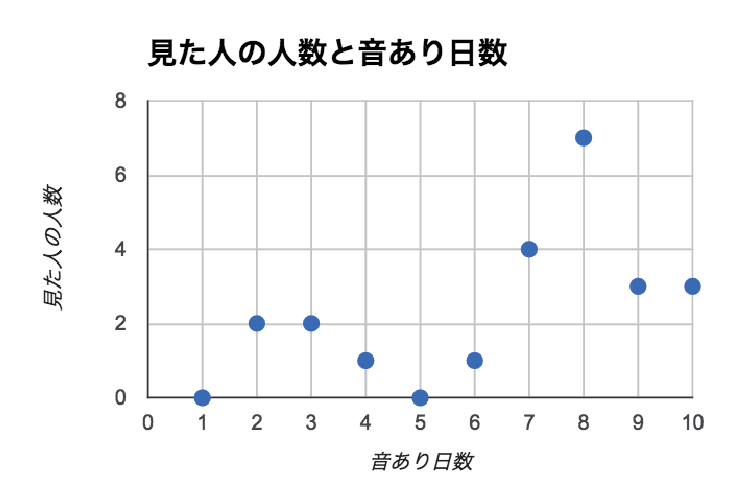
\includegraphics[width=12cm]{eps/experimentDates.eps}
\caption{DreamDateの試用期間と明晰夢を見た回数の相関図}
\label{dates}
\end{center}
\end{figure}

実験を通して明らかにできたことを以下にまとめる。
\begin{itemize}
\item 被験者の思い出とより直接的な音を流すと明晰夢を体験できる確率があがる
\item DreamDateの使用期間が長いほど成功確率が上がる
\end{itemize}

\subsection{DreamDateの有効性を高めるためにできること}
DreamDateには思い出に直結する音を登録する:\\
 本研究を通して、DreamDateで体験できる仮想体験には限界があるということがわかった。人が夢を見るのは過去の記憶を整理するためである。そのためDreamDateでは思い出にない体験や情景を夢で再現することは困難である。実際に予備実験1では海の夢を見た被験者Aと被験者Cはどちらも過去に海に行った際の思い出を夢見たと答えた。一方で海にしばらく行っていない被験者Bは一度も海の夢を見なかった。また予備実験後に行った実験でも、自ら作曲した歌、演奏した曲、ダンスをした曲などの直接的な記憶にを連想させる音楽を流した被験者は10/30の確率、過去の思い出に関連した音楽を流した被験者は3/30の確率で明晰夢を体験したのに対し、自分は体験していないが映画などを通して間接的に体験した記憶にまつわる音楽を流した被験者は7/30の確率でしか夢を見ることができなかった。この結果は被験者の記憶と関連性の高い音を流すと効果が出やすいということが示唆する。よって、明晰夢システムとしてDreamDateで選ぶべき音は思い出に直結する音である。\\

起床時の生活習慣を変える:\\
 全てのユーザが思い出とうまく連携した音を考え付くわけではない。実際に被験者 1 は音楽にあまり関心がなく、特に思い出に残る音・音楽がなかった。そこで最後に行った実験では被験者1に日常生活の中でコーヒーを飲む時に必ず特定の音楽を聴く習慣をつけてもらうことにした。すると図\ref{experiment3}でもあるように実験の最終日でその夢を見ることができた。Ivan Pavlovは条件反射という考え方を提唱している\cite{pavlov}。Pavlovは実験の中で犬に餌を与える前に決まってサイレンを鳴らし続けた結果、サイレンを鳴らすと犬の唾液量が増える現象が起きたと説明している。犬がサイレンを聞くと餌のことを反射的に考えたためだというのが通説である。被験者1は最後の夜に一度夢を見ただけのため、被験者の人数を増やしてさらに精度を上げた実験をする必要があるが、レム睡眠中に音楽が鳴ったことで被験者1に条件反射が働きコーヒーを飲む夢を見た可能性があると考えれる。もし仮説が正しければ、旅行をするときに特定の曲を意識的に繰り返し聴くことで旅行が終わった後もDreamDateでその音を流し旅行での想い出を夢で再生することが可能になる。但し、ある夢を見るために生活のあり方を変えるのは相当高いモチベーションを持ったユーザに限られるだろう。\\

音を流すタイミング:\\
 睡眠中に被験者が起きてしまうと意味がないのだが、ユーザがもっとも起きやすいとされているのはレム睡眠中である\cite{レムノンレム}。そこで予備実験の後に行った実験では被験者を起こさないで明晰夢を促す方法を検証するために音を流すタイミング別に実験結果を検証した。するとレム睡眠中ずっと音を流すのに比べて最期のレム睡眠時にのみ音を流した場合の方が明晰夢を体験できる確率が上がったことが図\ref{result}から読み取れる。この結果からユーザの睡眠が害される可能性を低めるためにタイミングとしては、レム睡眠中ずっとではなく音を流すのは起きる直前のレム睡眠の時が最適であるということが分かった。

\subsection{明晰夢で好ましい仮想体験を味わうことはできるのか} 
DreamDateが提供できる仮想体験の限界:\\
 DreamDateによって全ての被験者が思い出に関連した明晰夢を体験することができた。しかし体験できる夢の内容は限定されている。第2章でオンラインアンケートを行った際に空を飛ぶ夢、サイエンス・フィクションを連想させる夢、アイドルと遊ぶ夢、卒業論文の進め方を教えてくれる夢などそれまでに体験したことのない夢を見たいと答えた人がいたが、そのような夢を見るにはHMDを使った方が適切である。一方でDreamDateで体験可能なのは被験者の思い出に由来した夢である。夢を見ている際、脳は脳が記憶の整理を行っている\cite{Zhang}。DreamDateでは脳の習性を利用して思い出と関連性のある音を流すことで、明晰夢を促す手法をとった。実験では 7人の被験者全員が明晰夢を体験することができた。予備実験2で被験者Cは希望であった遠距離恋愛中の交際相手とデートしたいという要望を実現させることができ、起床後もその体験を忘れずに覚えていた。そして物理的制約を超えて交際相手から手紙が届く夢やデートしている夢を見ることで幸せな気持ちを味わうことができた。DreamDateはVRコンテンツを制作するスキルや時間のないユーザでも気軽に始められるこという利点はあることが証明された。

明晰夢の副作用:\\
 被験者Cは起床後現実は違うということを悟り残念に思う気持ちを味わってしまったとも答えた。明晰夢の副作用についてはDenysがMnemonic Induction of Lucid Dreams (The MILD Technique) で過度に明晰夢を行うと、夢に依存して現実逃避したい気持ちにかられたり睡眠後疲れが取れない現象が起きると説明がある\cite{LaBerge}。よってDreamDateを使うユーザにはあらかじめその現象が起きる可能性があることを了承した上で提供する必要性がある。